\documentclass[pdftex,12pt,a4paper]{report} 

% Document settings

\usepackage{fullpage}
\usepackage{cite}
\usepackage{datetime} 
\usepackage{geometry}
\usepackage[pdftex]{graphicx}
\usepackage{verbatim}
\usepackage{todonotes}
\usepackage{array}
\usepackage{capt-of}
\usepackage[parfill]{parskip}
\usepackage{underscore}
\usepackage{url}
\usepackage{listings}


 \usepackage{courier}
 \lstset{
         basicstyle=\footnotesize\ttfamily, 
         numberstyle=\tiny,      
	language=Java,
 }
 \lstloadlanguages{
         Java
 }


\geometry{verbose,lmargin=3cm,rmargin=3cm}

\newcommand{\HRule}{\rule{\linewidth}{0.5mm}}

\begin{document}

\title{Computer Music Improvisation - A Grammatical Approach For Blues}
\author{Cliff Sun (chs09)}
\date{January 2013}
\maketitle


\setcounter{tocdepth}{2} % Set the depth of toc indexing

\tableofcontents

\pagebreak

\renewcommand*\thesection{\arabic{section}}

% \section{Acknowledgements}

% acknowledge

\pagebreak

\chapter{Introduction}

\section{Project Introduction}
Improvisation is often seen as a human activity, especially in the domain of music. Genre's such as Jazz and Blues are heavily based on the performer improvising on a set form. Improvisation itself is essentially just a set of skills and techniques with rules that need to be learnt just like any other activity. So it is not to say that a computer can not 'improvise'. The aim of this project is to be able to model and replicate such music improvisation using a computer. The area of computational creativity in music has been explored before and is still ongoing, and we hope that this project can provide a new approach for computer music improvisation.

\paragraph{Improvisation vs Composition}
Music improvisation can be defined as the creative activity of immediate composition, or 'Composition on the fly'. In the case of our project when we talk about composition, it means the same thing as improvisation.

\section{Computational Creativity}
The project comes under the area of computational creativity, and it's uses and contributions are fairly novel. Computational creativity tries to answer the main question of whether a computer can be creative. Much work has been done in the field of generated visual art with tools and programs such as Simon Colton's Painting Fool \cite{website:paintingfool} and Harold Cohen's AARON \cite{website:aaron}. The work done in the area of computational creativity helps us to answer and theorise as to how we perceive creativity and whether by making a computer 'creative' it makes it seem more human-like.

\section{Blues Improvisation}
Blues is one of the most common genres that relies on performer improvisation. Performers of this genre tend to play a musical instrument (including voice) on top of an accompaniment with a well defined structure/form. The blues form itself is often defined by its 12 bar chord progression (commonly called 12 bar blues) which is essentially a standard harmonic chord progression of 12 bars in a standard 4/4 time signature. Table 1.1 below shows the chords for the general 12 bar blues form, with I7 referring to the harmonic seventh Tonic chord. Chord IV refers to the 'dominant' chord (4th degree) and Chord V refers to the 'dominant' chord (4th degree).


\begin{table}[here]
\centering
\newcolumntype{C}{>{\centering\arraybackslash}m{23pt}<{}}
\begin{tabular}{|*{12}{C|}}
  I & I or IV & I & I7 & IV & IV & I & I7 & V & V or IV & I & I or V
\end{tabular}
\caption{12 bar blues chord progressions}
\label{12 bar blues}
\end{table}


\begin{table}[here]
\centering
\newcolumntype{C}{>{\centering\arraybackslash}m{23pt}<{}}
\begin{tabular}{|*{12}{C|}}
  I & I & I & I & IV & IV & I & I & V & IV & I & I
\end{tabular}
\caption{12 bar blues simplified chord progression}
\label{12 bar blues}
\end{table}


Table 1.2 gives us one possible (and simple) chord progression for 12 bar blues in which we will basing our improvisation upon. 


\subsection{Blue Notes} What really gives the blues genre it's characteristics are the 'blue notes'. These are notes which are played at a lower pitch (flatter) than that of the major scale (usually one semitone lower on piano). The notes which are 'flattened' are the \textbf{third}, \textbf{fifth} and \textbf{seventh} notes of the major scale.
There are theoretical reasons for the introduction of 'blue notes' which we won't go into detail here. But essentially these 'blue notes' allow for moments of expression in blues melodies. 

\subsection{Blues and Pentatonic Scales}
Blues scales include the blue notes that we've mentioned above, these scales give the performer a set of notes to improvise with and gives the music the characteristic 'blues' feel to it. Blues scales are generally based on the major/minor pentatonic scale. A pentatonic scale is a scale of five notes (compared to seven notes in regular major/minor scale) and is widely used in music across the world. The most common blues scale (and the one we are going to be basing our improvisations on) is the blues minor scale which is based on the minor pentatonic scale (see Figure \ref{fig:cminorpentatonicscale}) with a sharp 4th note (or a flat 5th note, both are equivalent). In Figure \ref{fig:cminorbluesscale} we can see the blues minor scale includes all the blue notes; E(3rd degree) flat, G(5th degree) flat and B(7th degree) flat.


\begin{figure}[here]
  \centering
  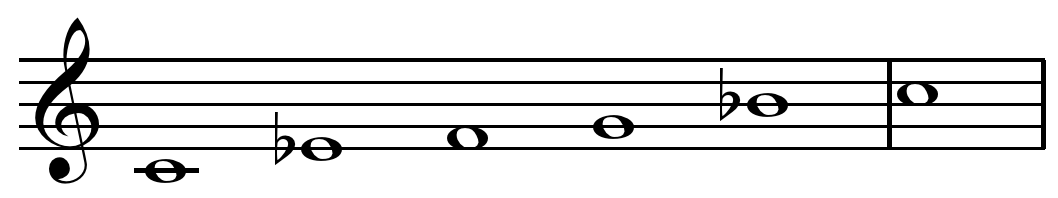
\includegraphics[scale=0.3]{figure/minorpentatonicscale.png}
  \captionof{figure}{C minor pentatonic scale}
  \label{fig:cminorpentatonicscale}
\end{figure}

\begin{figure}[here]
  \centering
  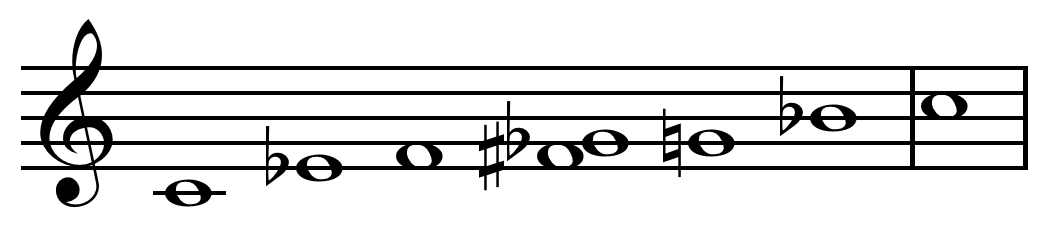
\includegraphics[scale=0.3]{figure/bluesminorhexatonicscale.png}
  \captionof{figure}{C minor blues (hexatonic) scale}
  \label{fig:cminorbluesscale}
\end{figure}


\section{Computer Improvisation For Blues}
Using the characteristics of blues music, we can limit our musical domain which simplifies the overall problem. Our aim is to be able to generate/improvise blues melodies on top of a standard 12 bar blues progression using a computer. Musical improvisation also covers improvisation/variations for the accompaniment as well. A grammar for improvising accompaniments in 12 bar blues/jazz is covered in Steedman's paper 'The Blues and the Abstract Truth: Music and Mental Models' \cite{steedman96}. However in this project we are only considering improvisations in the melody.

The above explanations on blues scales and chord progression only concerns the pitch characteristics of blues music. The issue of rhythm and structure is just as crucial in defining blues music and has yet to be discussed. There are many different approaches to such a problem and many of them have involved a statistical/machine learning approach. We propose a more grammatical approach to composing and generating blues melodies which will allow us to create well-defined structures and rhythms for blues melodies. The next chapter explains this in detail. In addition we hope to include a genetic/evolutionary part to the improvisation which will allow the computer to improvise in a more human-like way, i.e. variation and invention of new melodies/licks using previous/current knowledge.

\paragraph{Keys}
For simplicity, everything we do (melody generations/chord progressions) will be done in the key of C. We will be basing improvisations on the C minor blues scale and use a simplified 12 bar blues progression in the key of C.

\section{Related Works}
Work on computer music improvisation dates back 20-30 years or so. One famous example of computer generated music in general is David Cope's EMI (Experiments in Music Intelligence) which produces music in the style of various composers (using existing works as input sources). In terms of computer improvisation for jazz and blues music, there have been numerous machine learning approaches. One such piece of work is entitled 'Finding temporal structure in music: Blues improvisation with LSTM recurrent networks' By Eck and Schmidhuber (2002) \cite{eck02}. In addition Belinda Thom's Band-out-of-a-Box (BoB) describes an interactive soloist which can improvise with another performer using unsupervised learning in 'Unsupervised Learning and Interactive Jazz/Blues Improvisation' (2000) \cite{thom2000}.

Other works regarding grammatical approaches for music improvisation include approaches based on string rewriting grammars (L-systems) in 'Grammar Based Music Composition' by McCormack (1996) \cite{mccormack96}. In addition 'A Grammatical Approach to Automatic Improvisation' by Keller and Madison \cite{keller07} introduces a formal grammar for music improvisation in which we will be basing our work on (see more below).


\section{Project Plan and Milestones}

The main purpose of the project is to find and improve on grammatical approaches for the improvisation of blues music. We propose the following plan for the project along with the rough dates for expected completion. 

\subsection{Milestone 1 - Non-grammatical Random Improvisation}
\emph{Completed - End of December} \\
To start off we want to be able to experiment with blues improvisation using random notes from the blues scale. We can also generate equal or mixed durations. By using probabilistic methods we can also make melodic sequences sound better (constraining direction and intervals). This milestone also covers the implementation of the foundation for the project, such as representation of musical notes and phrases in abc notation

\subsection{Milestone 2 - Implementation of Blues Grammar}
\emph{Expected Completion - End of May} 
\begin{description}
\item[Initial Grammar Implementation]
'A Grammatical Approach to Automatic Improvisation' by Keller and Madison \cite{keller07} provides a grammatical approach for improvising jazz/blues melodies. Our aim is to reimplement the grammar and make adjustments to fit on 12 bar blues. Improvements and changes to the grammar can also be made to improve the result of the improvisation. 
\item[Terminal to Melodic Sequence]
In addition we aim to implement a system which appropriately chooses the best melodic notes from a terminal sequence (see in Chapter 2). This is not described in Keller's paper but is essential for producing better sounding melodies.
\end{description}

\subsection{Milestone 3 - Genetic Algorithm Extension}
\emph{Expected Completion - Mid-June} \\
On top of the grammatical approach discussed in milestone 2, we hope to be able to extend the capabilities of generating blues melodies by using genetic algorithms to manipulate the parse trees for blues grammar. This is in hope of producing a more interesting and varied sound for blues melodies.


\pagebreak

\chapter{Background - Grammar For Blues}

\section{Introduction}
In this project we propose a grammatical approach for generating blues melodies. Grammars have been used in other works in the field of computer music improvisation (see Chapter 1 - Related Works). More dominant however is the use of machine learning techniques for music improvisation/generation. 'Finding temporal structure in music: Blues improvisation with LSTM recurrent networks' By Eck and Schmidhuber (2002) \cite{eck02} is a more recent example of using LSTM networks to generate blues melodies. However there is a need for a training set and the result is affected by the quality of the training set. Using a grammar means that we don't need to encode a training set or input set and can directly influence our resulting sound.

\section{Grammars and Music}
Grammars enforce structures within music and such a linguistic approach seems suitable for the 'call and response' nature of African-American influenced music such as blues. We can compare a line of melody to a sentence in natural language. For example a sequence of notes and the rhythm that they occur in gives a melody it's own character and meaning, like a sentence in natural language. However in music there are no semantic rules in terms of the melody, it is entirely up to the listener/player as to how they interpret it. This is where a grammar comes in, grammars are structural rules that govern the composition of 'sentences' (in the case of natural language) and such grammars are not concerned with the semantics of the sentence. Therefore a well-defined grammar for blues music should be able to produce well-structured blues melodies.


\section{Initial Non-Grammatical Approach}
Before diving into a grammatical approach for blues melody improvisations, we decided to explore some simple ideas regarding probabilistic generation of notes in a sequence. Below are two simple approaches that we took. Note that we could easily classify these approaches with a simple grammar, however the point of introducing a grammar is so that we can defined structure and rhythm in our melodies, so for now we say that the first two simple approaches/implementations are not a 'grammatical' approach.

\subsection{Simple Probabilistic Generation (with fixed duration)}
We decided to make a quick music improvisation tool which uses probabilities to pick the next note in the melody. We kept the duration constant (a quaver/eighth note) and kept the range within one octave. An example of the generation is shown below in Figure \ref{fig:randomgeneration}. We designed it so that the probability that we choose the next note has an inverse relation to the interval of the note itself. I.e. the probability is of choosing an adjacent note in the blues scale is highest, with the probability for choosing a note that is 2 notes apart lower. In addition we made it so that the probability that we choose a note so that sequence is going in the same direction is higher than choosing a note that changes the direction of the sequence. For example if we had an F (natural) followed by an F\#, the probability of choosing G is higher than choosing an F (natural) (both one note interval from F\#).

\begin{figure}[here]
  \centering
  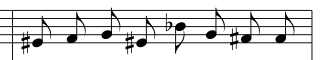
\includegraphics[scale=0.7]{figure/randomgeneration.png}
  \captionof{figure}{Probabilistic generation for a blues sequence}
  \label{fig:probabilisticgeneration}
\end{figure}

In the figure above we can see that a probabilistic random generation of notes with some constraints yields a fairly decent result. The notes are all part of the blues scale and so sound acceptable as a blues melody, however it lacks structure and rhythm as all the notes are of the same duration. 

\subsection{Probabilistic Generation With Mixed Durations}
To add some rhythm to the melody we decided that we could randomly choose duration lengths when we chose the next note. In our implementation we limited ourselves to semiquaver (16th), quaver (8th), and crotchet (quarter) notes. The idea was to introduce some style of rhythm to the music in the hopes of trying to make the melody fit into the blues criteria.

In Figure \ref{fig:randomgenerationwithdifferentdurations} we can see that choosing a random duration can give decent results. In our case we have an example of syncopation with the Eb quaver being played half a beat after the second beat. This sounds interesting and much more like blues music than in the previous example (in section 3.1). However not all bars generated look like this, some don't sound pleasing at all and some sound wrong rhythmically. As we are generating random durations, we are generating random rhythms and sequences and we may occasionally get a good melody, but a lot of the time we get bad or awkward rhythms. 

\begin{figure}[here]
  \centering
  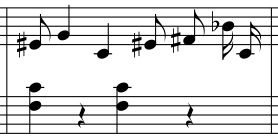
\includegraphics[scale=0.6]{figure/randomgenerationdifferentdurations.png}
  \captionof{figure}{Probabilistic generation with varying durations}
  \label{fig:probabilisticgenerationwithdifferentdurations}
\end{figure}


\section{Adding a Grammar For Blues}
The initial approaches are promising and give us a good foundation to build upon. If we randomly choose notes from a blues scale, they generally sound acceptable/good in terms of the pitch. However we have identified that some of the melodies/bars do not sound good rhythmically, i.e. they either don't sound good at all, or don't have the blues characteristics. We can see now that the rhythm of the notes is just as important as the pitch of the notes. 

In Keller and Madison's paper \cite{keller07}, a comprehensive grammar for blues is specified with excellent results. In particular a stochastic context-free grammar is used, where production rules of a context-free grammar are augmented with a probability/weighting. By using ideas from this approach we hope that we can create a more comprehensive grammar with more scope for variations. The terminal alphabet for the grammar is classified into different types of 'tones'. A grammar can use these different types of tones to form a melodic sequence. The classification of different tones is very much applicable to blues/jazz improvisation where knowledge of how to put these different types of tones together mean a better sounding melody is formed. In our previous non-grammatical examples, we use only notes from the blues scale. Though they sounded fine musically, using such a small set of notes means that the melody sounds flat and uninteresting for the most part. It is actually valid in music to use notes that aren't part of the scale, they can be used as a 'passing note' for example and as such makes the melody sound more interesting and complete. An article by Keller entitled 'How to Improvise Jazz Melodies' \cite{jazzkeller} talks about different methods for improvising blues/jazz melodies. The article provides many different methods and guidelines for improvising jazz/blues melodies. The above mentioned paper \cite{keller07} however only uses a few of these guidelines (albeit the most important ones). The classification of notes/tones are as follows:

\begin{description}
  \item[Chord Tones (\textit{C})] are tones (notes) which belong to the current chord we are improvising on top of.
  \item[Colour Tones (\textit{L})] are auxiliary tones for the current chord which sound correct musically when played with the current chord as an accompaniment. In particular, colour tones do not belong to the notes in the chord. 
  \item[Approach Tones (\textit{A})] are also notes which aren't in the chord (not the same as colour tones either) but they make good transitions to chord-tones or colour tones. These are also sometimes known as 'passing notes' where such a note can be placed between two chord/colours to make the melody seemed less disjointed. It is often bad practice however to place two approach tones next to each other.
  \item[Other] tones which don't belong to any of the above. These may include a rest \textbf{(\textit{R})}, or a scale tone \textbf{(\textit{S})} (a tone in the scale which works musically with the accompanying chord).
\end{description}

The issue we were concerned with before was whether we should deal with pitches of notes separately from the duration of the note. We have an option to create a grammar just for the rhythm of the melodic sequence. However randomly picking notes from the scale will not give us a result as good as the one in Keller and Madison 2007. The idea of chord, colour and approach tones provides us with a much better method of generating better sounding melodies.

\subsection{Context-Free Grammars}
The grammar described above is a context-free grammar. A grammar is considered context-free if the rules (production rules) of the grammar can be applied, i.e. the non-terminals can be written, without being dependant on the surrounding symbols. The majority of natural languages can be said to be based on context-free grammars. In addition we can say that the implementation of such a grammar for blues music is similar (and should be similar) to the implementation style of context-free grammars for random sentence generators. 

Context-free grammars are defined by the 4-tuple (V,$\Sigma$,R,S):

\begin{description}
  \item[V] - a finite set of \emph{variables}(non-terminal characters). Each variable essentially represents a different way to put together different families of notes and durations.
  \item[$\Sigma$]  - a finite set of \emph{terminals} which contain the actual content. In the case of our grammar, the terminals represent the type of tones/notes in the sequence.
  \item[R] - a set of production \emph{rules} in the form of A $\rightarrow$ b, where A is a variable $\in$V and b could be a sequence of variables and/or terminals.
  \item[S] - the starting variable/symbol used to represent the whole sentences where S$\in$V.
\end{description}


We start with starting variable S and expand the right hand side of the rule for S using other production rules. Expansion occurs by replacing variables in the sequence with the right hand side of the rule for that variable. We do this until the final result is a sequence of terminals only.

\subsubsection{Stochastic Context-Free Grammar}
The grammar that is defined in Keller's paper \cite{keller07} is a context-free grammar with probabilities, a stochastic/probabilistic context-free grammar. Each production rule has a probability associated with it which determines the likelihood of which production rule to use (if there are more than 1 with the same variable on the left hand side). The grammar specified below is such a grammar.

\subsection{Blues Grammar}
We aim to implement the grammar described in the paper by Keller \cite{keller07} and extend it or make improvements to it. The grammar itself is essentially a set of production rules which represent different rhythmic phrases with families of tones and their duration as the terminals. At the top level, we have the production rules P(n) $\rightarrow$ ... where n is the length of the melody generated in quarter/crotchet beats and n $\in$ 1..N:

\begin{verbatim}


P(0) -> empty [1]
P(1) -> Q1 [1] 
P(2) -> Q2 [1] 
P(3) -> Q2 Q1 [1] 
P(n) -> Q1 P(n−1)  [ .4 ]
P(n) -> Q2 P(n−2)  [ .4 ] 
P(n) -> Q4 P(n−4)  [ .2 ]

\end{verbatim}

A P variable takes in argument n, which limits the generation of the melody to fit n beats. We could also have a recursive grammar which expands until it reaches a set limit, but we may end up truncating a phrase which is not preferred. The values in the square brackets denote the weights for choosing a particular rule. It is worth noting that for the rules above, the weights are the same as probabilities (they add up to 1, so for P(n):  0.4+0.4+0.2 = 1), however it is not a requirement. The weights will will be normalised so that the actual probabilities are worked out.

The rest of the rules are taken from the aforementioned paper. We have rewritten the names of variables so that the numbers which follow a letter (i.e. Q4, V1, N/2 etc) denote the length of the notes generated (in quarter/crotchet beats). For example all the terminal sequences that can be generated from variable Q4 will have a total length of 4 crotchet beats. In addition, the number of beats that V/2 produces is half a beat (and also any other variable with /2). The specification of the grammar in Keller's paper \cite{keller07} is slightly inconsistent in the variable naming convention and can cause confusion. Therefore the rules (with new renamed variables) are as follows:

\begin{verbatim}


Q4 -> Q2 V1 V1  [0.52]
Q4 -> V/2 N1 N1 N1 V/2  [0.01]
Q4 -> V1 Q2 V1  [0.47]

Q2 -> N2  [0.06]
Q2 -> V1 V1  [0.6]
Q2 -> V/2 N1 V/2  [0.12]
Q2 -> H3/2 N/2  [0.16]
Q2 -> ({3} H1 H1 H1)  [0.06]

Q1 -> C1  [1]

V1 -> N1  [0.22]
V1 -> V/2 V/2  [0.72]
V1 -> ({3} H/2 H/2 H/2)  [0.05]
V1 -> ({3} H/2 H/2 A/2)  [0.01]

V/2 -> N/2  [0.99]
V/2 -> H/4 A/4  [0.01]

N2 -> C2  [1]

N1 -> C1  [0.5]
N1 -> L1  [0.2]
N1 -> S1  [0.5]
N1 -> A1  [0.01]
N1 -> R1  [0.25]
N/2 -> C/2  [0.4]
N/2 -> L/2  [0.2]
N/2 -> S/2  [0.4]
N/2 -> A/2  [0.01]
N/2 -> R/2  [0.1]

\end{verbatim}

In the N-variables, C, L, S, A and R are terminals in the terminal alphabet. They are shorthand for the families of tones that we've described at the beginning of the section. The grammar itself contains 4 distinct levels / types of variables:

\begin{description}
  \item[N-variables] - e.g. N2, N1 and N/2. These variables are at the bottom of the tree and their rule is always rewritten as a single terminal with the same length as the variable (see above).
  \item[V-variables]  - e.g. V1 and V/2. These are intermediate variables that describe small rhythmic sections. They allow the specification of different ways of making up a certain number of beats. For example we could add rules for V1 to represent more possible phrases, such as [V1 $\rightarrow$ H/4 N/2 H/4] if we wanted to add more variety to the music. They use the N-variables above to construct the sections. Note that the H-variable is a terminal which represents a \textbf{helpful} tone and refers to any of the Chord (\textit{C}), Colour (\textit{L}) and Approach (\textit{A}) tones.
  \item[Q-variables] - e.g. Q4, Q2, Q1. These are top level variables which essentially combine smaller sections/phrases to produce the larger sections. 
  \item[P-variable] - e.g P(n), the starting variable (as seen previously).
\end{description}

Again each rule has a probability associated with it and the above probabilities are taken from the above mentioned paper. The probabilities themselves play a large role in how the resulting melody sounds and at the moment can only be adjusted by the user.

Each unique derivation for each duration we generate for (the n in the P(n) starting variable) has its own unique parse tree. Figure \ref{fig:Q2parsetree} shows a partial parse tree just for Q2, which is already fairly comprehensive. We can see that the overall probability for generating a terminal sequence \emph{C1 C1} or \emph{C1 S1} from Q2 is 0.6x0.22*0.22*0.34*0.34= 0.00336. It is worth noting that many more melodies can be created with one particular terminal sequence, which we will discuss below.

The implementation of the above grammar will give the same results as in Keller's paper \cite{keller07}, indeed changes and enhancements may be made along the way to try and improve the result. 
It would also be better if we could allow users to adjust the grammar themselves to produce different melodies, for example a more complex grammar would perhaps produce a more complex melody. 

\begin{figure}[here]
  \centering
  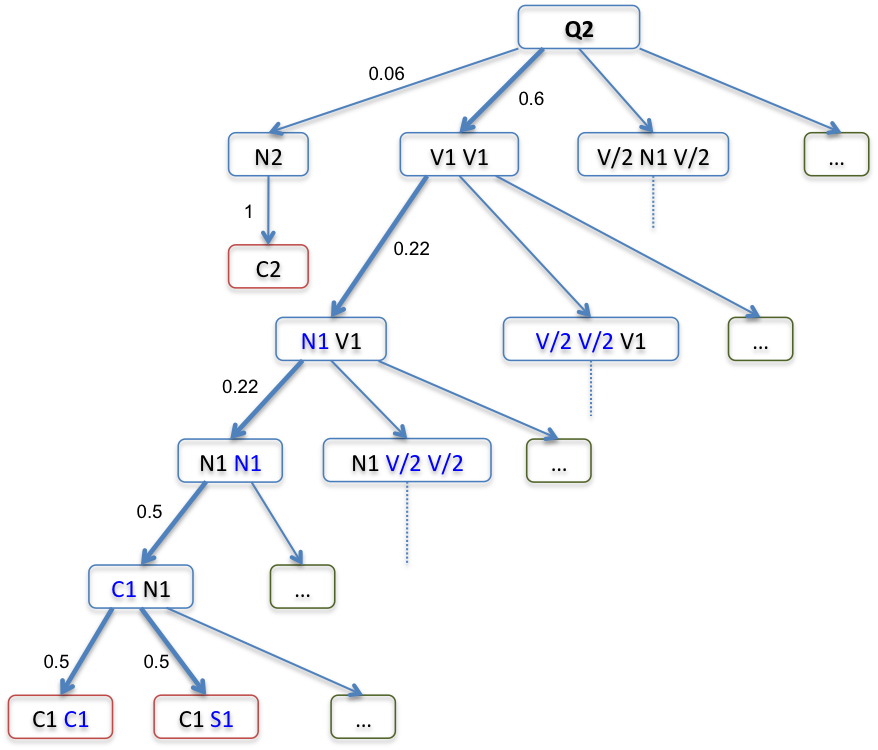
\includegraphics[scale=0.8]{figure/Q2parsetree.png}
  \captionof{figure}{Parse tree for Q2}
  \label{fig:Q2parsetree}
\end{figure}

\subsection{Terminal Sequences to Melodic Sequences}
As we've discussed previously, the grammar above generates a terminal sequence of types of tones and durations. Additional work needs to be done in order to produce a sequence of actual musical notes. An example terminal sequence that may be generated for P(4) $\rightarrow$ Q2 Q2 may be:

\begin{verbatim}
C/2 L1 H/4 A/4 H3/2 S/2
\end{verbatim}

We could generate many melodic sequences from the terminal sequence alone. However we would prefer to generate better sound melodies if possible. To do this we would have to introduce constraints when choosing actual musical notes from the families of tones, otherwise we may end up with a melody that sounds as random as our non-grammatical attempts. To do this we refer to Keller's article 'How to Improvise Jazz Melodies' \cite{jazzkeller}. Here are some possible ways we can constrain the selection of notes to ensure a better sounding melody:

\begin{description}
  \item[Know scales that go off the chords] scale here refers to a set of notes, rather than a sequence. If we know what scale works for the current chord, then it can help constrain the choice of tones so that the melody is closer to the scale.
  \item[Intervals between notes] smaller intervals often sound more pleasing than large intervals, however it is good to have both. If our intervals are too big then the melody will sound quite discordant. However alternatively 'skipping' notes can sound good if combined with a direction change (see below) and can give a zig-zagged effect.
  \item[Change direction] if we have a sequence of small intervals (scale-like sequence) we may want to change direction at some point to provide variety and make the melody sound more interesting. We don't want to do this too often however as it may sound disorientating.
  \item[Use of enclosures] similar to direction changes, we can approach a note from both sides alternatively. This involves making sure intervals get smaller and also direction changes occur. Enclosures work better if the target tone is a chord tone.
\end{description}

By implementing these musical features, we can avoid awkward note combinations and optimise the melodic sequence from the terminal sequence.


\chapter{Genetic/Evolutionary Algorithm Extension}

\section{Approach}
The problem with a grammar is that it has a finite search space, this is more noticeable with a smaller grammar. The music generated from the context free grammar in Chapter 2 will always resemble the same style and more importantly the same complexity. In reality, a human musician learns and continually improves over time, for example they may discover a new style to play music or find a new phrase/jazz lick that sounds better. They also improve their skills and  If we want our computer to be able to improvise like a human then we would need for it to 'evolve'.

The idea in this is that we would like to be able to allow our program to continue to produce 'new' music and improve on our improvisations/compositions. We can do this using evolutionary techniques such as selecting fragments/phrases from some melodies, then possibly add some sort of 'mutation' to it and recombining them together to form a new melody. The application of genetic algorithms may be useful for such a task. In particular interactive genetic algorithms, where the fitness function is the user or listener, due to the difficulty of judging musical quality computationally. However it may be possible to determine fitness based on simple melodic and rhythmic characteristics. 

Essentially we have to define our crossover function, our mutation function and our fitness function.

\section{Example}
A simple example would be show the user a selection of melodic sequences. The listener would indicate which sections sound good, or which sections sound bad (fitness function/evaluation). We can then perform crossovers of pairs of sequences to produce children. Crossovers could include swapping phrases around at the same place in the piece. We could then perform mutations on the child sequences such as altering the rhythm of a section. We would allow the fittest/best sounding sequences to be used more often for crossover, thereby producing better child sequences.

Crossover may also be done using terminal sequences (chord, colour approach tones etc) and not the actual sequence of notes. The reason for this is that swapping phrases of actual notes may result in disjointed sequences.

\chapter{Implementation}

\section{Overview}
The implementation of the blues improvisation using the grammar specified above will be primarily done in Java. Development will be done in the Eclipse IDE which provides good support including refactoring tools and auto-completion. Build management of the project is handled by Apache Maven, which manages dependencies and plugins required for the project. 

\section{Representation of Musical Score}
Initial work to add functionality to represent musical score as ABC notation (see section 3.4) using Java objects is also required. Although we could use existing libraries and tools to represent our musical score, it is more beneficial overall to create a small/light-weight set of classes which do exactly what we want. Currently the library is part of the overall project, however there are plans to move it into it's own sub-project for uses externally. This way, users can use this library to create notes and scores and print them as ABC notation.

For example in Figure \ref{fig:abcnotationexample}, if we want to represent the notes as ABC notation (disregarding headers and bar lines in the ABC file) then it would look like:

\begin{verbatim}
C _D ^F3/2 _B,/2
\end{verbatim}

Where '$\_$' represents a flat, '$\wedge$' represents a sharp, and the ',' represents a lower octave. The duration of the note (in this case in quarter/crotchet beats) is the number directly after the pitch of the note (C, D, E all have a duration of 1 quarter beat). So F\# and B both have /2 which indicates the duration is half of a quarter/crotchet beat, i.e. an eighth/quaver.

In Java, we would represent these notes by writing this code:

\begin{lstlisting}
MainNoteComponent middleCNote = 
      new MainNoteComponent(BasicNote.C);
TimedComponent middleCNoteQuarter = 
      new TimedComponent(middleCNote, Duration.quarter);

MainNoteComponent DFlatNote = 
      new MainNoteComponent(BasicNote.D, AccidentalShift.Flat);
TimedComponent DFlatNoteQuarter = 
      new TimedComponent(DFlatAboveMiddleCNote, Duration.quarter);

MainNoteComponent FSharpNote = 
      new MainNoteComponent(BasicNote.F, AccidentalShift.Sharp);
TimedComponent FSharpNoteDottedQuarter = 
      new TimedComponent(FSharpNote, Duration.dottedQuarter);

MainNoteComponent BFlatBelowMiddleCNote = 
      new MainNoteComponent(BasicNote.B, AccidentalShift.Flat, -1);
TimedComponent BFlatBelowMiddleCNoteEighth = 
      new TimedComponent(BFlatBelowMiddleCNote, Duration.eighth);

\end{lstlisting}

To represent a bar with those notes (all in one phrase), we would write:

\begin{lstlisting}
Bar bar = new Bar();
StandardTimedComponentPhrase phrase = 
      new StandardTimedComponentPhrase();
phrase.addtoComponentList(middleCNoteQuarter);
phrase.addtoComponentList(DFlatNoteQuarter);
phrase.addtoComponentList(FSharpNoteDottedQuarter);
phrase.addtoComponentList(BFlatBelowMiddleCNoteEighth);
bar.addToBar(phrase);

\end{lstlisting}

By calling bar.getAbcRepresentation() we would get the abc representation of these notes as seen above.
These set of classes allow us to represent any note that we want, i.e. any duration, any octave and any accidentals. In addition we can also represent full scores as objects (with lists of bars). We can print any object out as ABC notation allowing us to use an external program/tool to play as MIDI or print the score.

\begin{figure}[here]
  \centering
  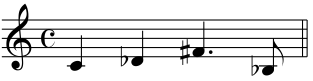
\includegraphics[scale=0.6]{figure/abcnotationexample.png}
  \captionof{figure}{Notes C, Dflat, Fsharp and Bflat}
  \label{fig:abcnotationexample}
\end{figure}

\subsection{ABC Notation}
ABC notation is a text-based music notation system which allows simple representation of musical scores. It is widely used in folk and traditional music and is ASCII based. There is support for the format including tools to convert abc notation to midi and to printable scores (as pdf's). More about the notation can be read on the website \url{abcnotation.com}.

\section{Grammar Implementation}
Numerous options have been explored for implementing the grammar (along with generation of melodic sequences) in Chapter 2, section 3.2. The main options are:

\begin{description}
  \item[Parser Generator Tools] such as ANTLR, which allows a context-free grammar to be specified using Extended Backus Naur Form and can generate lexers and parsers. It's main use is for generating a recogniser for a language define by the context-free grammar which checks the syntax of the input (a sample program in the specified language). ANTLR also has a maven plugin which can manage compilation of grammars.
  \item[External Languages] such as Python, or Lisp. These dynamic languages are useful for specifying a context-free grammar and generating sentences/sequences from the grammar. In particular in Lisp, a grammar can conveniently be expressed using s-expressions, a notation to represent a nested list hierarchy. Similarly a grammar can be represented using dictionaries in Python. 
  \item[Native Implementation in Java] would keep the codebase all in one language. The implementation of the grammar may not be as straightforward as in Python or Lisp as we would have to represent everything as objects in Java. This approach is feasible if the grammar is small. However if we were to expand the grammar in the future then this may not be the best option.
\end{description}

Currently the preference is to use an external language to represent the grammar and to do sequence generation. Python is currently preferred due to existing experience and knowledge of using the language. As we want to be able to use both Java and Python together, we can use Jython, an implementation of Python written in Java (i.e. it runs on the JVM). This way we can invoke Python code from Java, allowing us to store our specified grammar in Python and invoke Python methods to generate sequences from the grammar.

\chapter{Evaluation}

\section{Overview}
We hope that the project can contribute something towards the field of creative music improvisation. By building on existing grammatical approaches and by incorporating rules and techniques that we as humans learn when start learning how to play/improvise, we aim to be able to improve the standard of generated music so that it resembles human-played music. Additionally, we hope that such a tool can help and aid people who want to learn blues improvisation by generating simple melodies and phrases for them to practise with.  

\section{Measuring Success}
As we are improving on existing work laid out in Keller's paper \cite{keller07}, we could say that we can judge the success of the project by judging whether the new generated blues music sounds 'better' than the music generated by just the grammar alone in Keller's paper.

However it is not easy by any means to judge whether one piece of music is 'better' than the other piece of music. Of course we could say that being more pleasing to the ears is main criteria, but the auditory experience of a piece of music is subjective from person to person. We could use other criteria to judge the success of our efforts, for example we could say that the complexity of phrases and whether it matches up to phrases/licks in blues music composed by humans could form the basis of our assessment.

We would also want to compare whether our grammatical approach produces better results than a machine learning approach. It is also important to consider the scope of the music that we can generate using a grammar compared to using machine learning. For example machine learning techniques mean that a program can continually learn and train to produce better sounding / more complex pieces, whereas a grammar is constrained and limited in it's search space. 



\bibliographystyle{plain}
\bibliography{refs}

\end{document}


